\documentclass[a4paper, 12pt]{scrartcl}

\usepackage[utf8]{inputenc}
\usepackage[english, ngerman]{babel}
\usepackage[T1]{fontenc}
\usepackage{amsmath}
%für Bilder
\usepackage{graphicx}
%deutsche anführungszeichen
\usepackage{csquotes}\MakeOuterQuote{"}
%ränder
\usepackage[left=3cm, right=4cm, top=3cm, bottom=2.5cm]{geometry}
\usepackage[numbers, round]{natbib}
%spacing
\usepackage[onehalfspacing]{setspace}
%Abkürzungsverzeichnis
\usepackage[printonlyused, footnote]{acronym}
%Anzeigen der restlichen Verzeichnisse
\usepackage{tocbibind}
%Literaturverzeichnis
\bibliographystyle{alphadin}
%größere Schriftgrößen als 17pt
\usepackage{lmodern}
%bessere umbrüche
\usepackage{microtype}
%Bildquellen
\newcommand*{\bildquelle}{%
  \footnotesize Quelle:
}
%römische zahlen
\newcommand{\RM}[1]{\MakeUppercase{\romannumeral #1{.}}}
\makeatletter
\newenvironment{folding}{\endgroup}{\begingroup \def \@currenvir{folding}\edef \@currenvline{\on@line}}
\makeatother
\hyphenation{Schleu-sing-en Haupt-ein-kaufs-mö-glich-keit Nie-drig-preis-po-li-tik}

\title{Seminarfacharbeit}
\author{Toni Hausdörfer, Fabian Beez}
\date{27. Mai 2020}

\begin{document}
    \begin{titlepage}

    \raggedright
        Hennebergisches Gymnasium Georg Ernst\\
        Klosterstraße 2-4\\
        98554 Schleusingen
        
    \raggedleft\vspace*{-1.9cm}
        Jahrgang 2020/21
        
    
    \vfill\vfill\vfill\vfill\vfill\vfill

    \centering
        \LARGE\textbf{Seminararbeit}
        \vfill
        \large Onlinehandel und dessen Einfluss auf Kleinstädte und Dörfer im ländlichen Raum?\\[\baselineskip]\vfill
        
        von\\
        Toni Hausdörfer und Fabian Beez
    

    \vfill\vfill\vfill\vfill

    \raggedright
    Betreuende Lehrkraft:   Frau[?] Richter\\
    Abgabetermin:\\[\baselineskip]
    
\begin{tabular}[h]{|l|l|l|l|l|l|}
    \hline
    Bewertung & Note & Note in Worten & Punkte &  & Punkte \\
    \hline
    schriftliche Arbeit & & & & x 3 & \\
    \hline
    Präsentation & & & & x 1 & \\
    \hline
\end{tabular}

\vfill

\raggedleft
    Summe: \rule{1.5cm}{.4pt}\\
    Gesamtleistung nach \$ 61(7) GSO = Summe :2 (gerundet): \rule{1.5cm}{.4pt}\\[\baselineskip]\vfill\vfill\vfill
    \begin{tabular}{@{}l@{}}\hline
        Unterschrift des Kursleiters
    \end{tabular}
    
\vfill\vfill
\end{titlepage}

\newpage

    \input{exports/Fabian-Eidesstattlicheerklärung.tex}
     
\vspace*{5cm}
\section*{Danksagung}
Zuerst möchten wir uns bei all denjenigen bedanken, die uns während der Anfertigung dieser Arbei unterstützt haben. 
Dazu zählen in erster Linie alle Teilnehmer der Umfragen.
Ein besonderer Dank gilt dabei Frau Karin Richter, die uns als betreuende Lehrkaft unterstützte.
\newpage


    \tableofcontents 
        \newpage

    \section{Einleitung}
        %?: mode beetz, ..., in schleusingen schließen immer mehr läden und es werden kaum neue eröffent(abgesehen von restoraunnts). gleichzeitig wird der onlineeinkauf immer attraktiver



Onlinehandel spielt eine immer größer werdende Rolle im Leben von Menschen fast aller Altersschichten. Aufgrund des allmählichen Verschwindens von Geschäften im Gebiet um Schleusingen haben wir uns die Frage gestellt, welche Rolle der Verkauf von Waren über das Internet in unserem Landkreis spielt, und ob die Schließungen einiger Geschäfte auf den Rückgang der Nachfrage für lokale Einzelhändler zurückzuführen ist.

Im Rahmen unserer Arbeit werden wir das Zutreffen folgender Thesen einschätzen:
\begin{itemize}
    \item Der Onlinehandel führt zu einem allmählichen Aussterben von stationären Händlern im ländlichen Bereich.
    
    \item Es gibt Waren, die nicht/kaum online gekauft werden.

    \item Der Onlinehandel schafft weniger Arbeitsplätze als indirekt verringert werden.
\end{itemize}

Außerdem werden wir auf Basis unserer Ergebnisse ein Konzept entwickeln, wie die Nachfrage und der Verkauf von Waren in unserem Landkreis erhöht werden kann.

        \newpage
    
    \section{Historie}
        \subsection{Entstehung}
        \subsection{Entwicklung mit Blick auf Großfirmen wie PayPal}
        \subsection{Beeinflussung der Sozialstrukturen}
        \newpage
        
    \section{PayPal}
        \subsection{Entstehung und grobe Funktionsweise}
        \subsection{Entwicklung}
        \subsection{Einfluss auf die Gesellschaft}
        \newpage
        
    \section{Konsumverhalten}
             Amazon ist ein Onlineversandhändler, der eine breite Bekanntheit genießt und vor allem im europäischen Raum im Bereich des Onlinehandels einen großen Anteil ausmacht. Während Aliexpress in Asien und östlichen Teilen Europas und Ebay im Norden der EU stark vertreten sind, ist Amazon in Zentral-, Nord- und Westeuropa die Plattform mit dem größten Wert von Verkäufen\cite[S. 22]{EuroCommerce}. Außerdem macht Amazon bereits seit Ende 2017 mehr als die Hälfte der Verkäufe durch Drittanbieter aus\cite[S. 25]{Haendlerbund}. Dementsprechend werde ich in den folgenden Unterpunkten die Firma in Bezug auf ihre Entwicklung, die Auswirkungen dieser und der Konkurrenzfähigkeit zu lokalen Händlern analysieren und auf Basis der Erkentnisse Schlussfolgerungen im Bezug auf Schleusingen und des hildburghäuser Landkreis schließen.

        \subsection{Veränderungen im Konsumverhalten über die Zeit}
            \iffalse
Einteilung in: Online-Marktplätze + Online-Händler, Intermediäre, Kataloversender, stationäre Händler, Hersteller/Marken \cite{Graf}

entwicklung des kaufprozesses: graf:abbildung; 

https://edoc.sub.uni-hamburg.de/hcu/volltexte/2017/370/pdf/Ebert_Kirsten.pdf Anfang

änderung kaufablauf: \cite{Schaefers}
\fi

% ALLGEMEIN
Bis Anfang 2020 war das Konsumverhaten in Deutschland im Allgemeinen geprägt durch eine starkte Kaufkraft, z. T. dank dem 0\%-igen Leitzins der \ac{EZB}\cite[S. 49]{Ebert} - jedoch ist die Kaufkraft durch die derzeit vorherrschende Corona-Situation abgeschwächt worden\cite{BfWE}. 

Außerdem haben sich die Bedürfnisse innerhab der letzten Jahrzente stark geändert: statt gleichbleibenden, rationalen Käufen und Kaufmotiven in den 1950ern, die die Auswahl der gekauften Güter stark abhängig von der zur Verfügung stehenden Geldmenge machten\cite[S. 38]{Schramm}; herrscht heute ein deutlich dynamischeres Kaufklima:
\begin{quote}
"So beziehen jetzt zum Beispiel auch solvente Kunden ihre Lebensmittel aus dem Billigdiscounter, während  umgekehrt  einkommensschwächere  Schichten  zu  Luxusgütern  greifen."\cite[S. 43]{Nitt}
\end{quote}

Im folgendem werde ich Verkäufer aller Art ähnlich wie im Buch "Das E-Commerce Buch: Marktanalysen - Geschäftsmodelle - Strategien" unterteilen: in Online-Marktplätze, Online-Händler, Kataloversender, stationäre Händler und Hersteller\cite[S. 18ff]{Graf}. Dabei sind Online-Marktplätze eine Art Online-Vermittler zwischen Kunden und Verkäfer, Online-Händler bieten dagegen nur eigene, meist sehr spezialisierten Sortimente an. Kataloversender verhalten sich ähnlich: sie versenden ihr Sortiment direkt an Kunden. Stationäre Händler verkaufen im Gegensatz zu den genannten Verkaufstrukturen in Fillialen und sind am stärksten von den Änderungen der letzten Jahrzenten betroffen. Während sich die genannten Unternehmensarten meistens am Ende der Verkaufskette befinden, stehen Händler oft am Anfang: sie stellen Güter her und sind dementsprechend, insofern sie nicht selber verkaufen, auf weitere Unternehmen für Verkauf und Vermarktung angewiesen(ebd.). %vor und -nachteile?, beispielsunternehmen


\iffalse 
    VERÄDERUNGEN bzgl der Verkäuferstruktur
    
        individiuelle Produkte
        
        sozialer Aspekt: Einzelhandel
        
        Einzelhandel: erst anbieter, dann produkt; onlinehandel umgekehrt
            .> weil einfacheres vergleichen, mehrere läden lohnen sich nicht
            einzelhandel weniger preissensibel; jedoch ist onlinehandel vor allem in der Elektronikbranche konkurrenzfähig, sh. Media Markt\cite[S. 27]{Graf}
            ABBILDUNG GABLER S. 313
        Mutichannel: Onlinebestellung im laden abholen/zurückgeben, wenig mehrwert (S 37) 
            
        {
        Katalogversender bieten ab 2002 online an: +56\% Umsatz, S. 30f
        }
        
        Hersteller: "Powerseller" kaufen produkte von herstellern, verkaufen siedeutlich unter marktpreisen weiter -> probleme mit preisverfall S. 31
        schrecken aufgrund von biosherigen vertreib über fachhandel meist davor zurück, online-marktplätze einzurichten, vereinzelt(hugoboss.com) S. 34
        
        allgemein online: großes wachstum ab 2002 S. 32
            jüngere kaufen mehr online ein S 37f
            
    STEHENGEBLIEBEN: S 39
\fi

Zusätzlich hat sich unter vielen Konsumenten das Bedürfnis nach individiuellen und auf den Käufer angepassten Produkten gebildet\cite[S. 43]{Nitt}, was wahrscheinlich durch die extrem große Außwahl bei dem Online-Shopping hervorgerufen wurde. In diesem Aspekt kann der stationäre Einzelhandel schlicht nicht mithalten, da Raum für Produkte begrenzt und sehr teuer ist. 
\iffalse
> billig - strategie vorallem von amazon und alibaba

veranschaulichung eigene tabelle börsenwert einzelner unternehmen

Dabei gibt es auch unternehmen, die mehrere berieche nutzen, wie amazon
\fi

Allerdings hat der stationäre Handel noch einen bedeutenden Vorteil: den sozialen Aspekt. Dieser wird vermutlich mit fortschreitender Digitalisierung eine immer wichtigere Rolle spielen\cite[S. 50]{Ebert}.
\begin{quote}
"Als Mittel gegen Vereinsamung und Anonymisierung im Alltag wird die soziale Komponente beim Einkaufen [...] zunehmend an Bedeutung gewinnen."\cite[S. 43]{Nitt}
\end{quote}

            
        \subsection{Einfluss des Onlinehandels}% Überschneidung mit 7.2
            % 

            
        \subsection{Mögliche Probleme und Folgen}
            %zusammenfassung

%gegenseitige beeinflussung: showrooming-effekt: kauf online aufgrund von stationärere beratung -- kauf stationär nach onlinerecherche \cite[S. 21f]{evilcom}

%wie viele läden haben in schleusingen einen onlineshop?


\begin{folding} %stationärer Handel

Aufgrund der Verschiebung von Nachfrage und Bedürfnissen von Konsumenten in den letzten Jahrzehnten wird der stationäre Handel trotz Multichannel-Versuchen keine einfache Zukunft haben. So kann in vielen Fällen stattdessen direkt von Herstellern gekauft werden, die mittlerweile den Vertriebswegwechsel von \ac{B2B} zu \ac{B2C} weitesgehend hinter sich haben. 
Insbesondere in Thüringen steht es im Vergelich zum Rest Deutschlands dank der Kombination aus schlechter Kaufkraft und niedriger Bevölkerungszahl pro Fläche schlecht um den konventionellen Einzelhandel\cite[S. 29]{Nitt}. Dazu kommen demografische Änderungen, die insbesondere in der Mitte Deutschlands Probleme verursachen: so nimmt die Bevölkerung z. B. in Hamburg, trotz Schrumpfen der Bevölkerungszahl, zu - jedoch nicht in Hildburghausen, einer der Landkreise, die am meisten Bewohner verliert\cite[S. 32f]{Nitt}. 
Zum Glück einiger Vertriebe treffen diese schlechten Chancen nicht auf alle Branchen zu - der Lebensmittelvertrieb hat z. B. kaum Online-Konkurrenz[Umfrage]. Um in den restlichen Geschäftssektoren einen maximale großen Umsatz zu erzielen, sollte der konventionelle Einzelhandel aufgrund der alternden Bevölkerung, die meist noch stationär kauft, vorerst Investitionen für die wachsende Gruppe von Senioren und dementsprechend Erreichbarkeit o. ä. nutzen.

\end{folding}

\begin{folding} %Umweltverschmutzung

Zudem kommt immer öfter das Argument auf, dass der Wechsel zum Onlinehandel umweltschädlich sei, da mehr Lieferfahrzeuge unterwegs sind. Jedoch haben bereits die Autoren des "Evil Commerce [...]"-Buches diese These anhand einer Modellrechnung weitesgehend wiederlegt. Sie berechneten eine 90\%-ige Kraftstoffersparniss bei komplettem Umstieg zum Distanzhandel in Großstädten unter optimalen Bedingungen\cite[S. 25f]{evilcom}. Um genauerer Aussagen bezüglich des ländlichen Raumes zu treffen, werde ich die genannte Rechnung bzgl. Entfernung - da Einkaufszentren nicht berücksichtigt wurden - modifizieren und insofern erweitern, dass zusätzlich ein Einkauf in mehreren Geschäften nacheinander mit in Betracht gezogen wird.

\begin{itemize}

\item Im meiner Modellrechnung kaufen 100 Bewohner eines Dorfes in einer 4km entfernten Stadt ein. Sie kaufen im Durchschnitt in 3 von 10 Einkaufsmöglichkeiten ein, die je 500m voneinander entfernt sind. Dabei gehe ich davon aus, dass alle Kunden über eine 500m lange Straße innerhalb des Dorfes zu erreichen sind.

\item Wenn alle Bewohner stationär kaufen, legen sie im Durchschnitt eine Strecke von 

\begin{align}(250m + 4000m + 3 \cdot 500m + 4000m + 250m) \cdot 100 = 1000000m\end{align}

 zurück. Dabei nehme ich an, dass alle Bewohner denselben Ortsausgang benutzen und somit einen durchschnittlichen Weg von 250m zu diesem besitzen.

\item Wenn jeder Verkäufer jedoch die Güter an seine im Durchschnitt 30 Kunden versendet, müssten alle Lieferwagen zusammen eine Strecke von gerade einmal 

\begin{align}(4000m + 500m + 4000m) \cdot 10 = 85000m\end{align}

zurücklegen.
\item In dieser Darstellung hat der Distanzhandel eine ähnlich hohe Kraftstoffersparniss - 91.5\%. 

\end{itemize}
Zwar kann mithilfe dieses Modelles die These der Umweltverschmutzung auch auf dem Land im Allgemeinen wiederlegt werden, jedoch ist sie keine genaue Darstsellung der Realität, da viele Faktoren, wie z. B. die Retouranzahl, die beispielsweise in der Modebranche überproportional hoch ist, nicht beachtet wurden(ebd.).

\end{folding}

        \newpage
            
        
    \section{Auswirkungen des Oninehandels auf die Infrastruktur}
        \subsection{Vergangene Änderungen und Entwicklungen}
            \input{exports/Fabian/Infrastruktur-Vergangenheit.tex}
            
        \subsection{Mögliche Entwicklungen in der Zukunft}
            \input{exports/Fabian/Infrastruktur-Zukunft.tex}
            
        \subsection{Probleme mit dem Einfluss des Onlinehandles}
            \input{exports/Fabian/Infrastruktur-Probleme.tex}
        \newpage
        
        
    \section{Globaler Vergleich des Einflusses und der Entwicklung des Onlinehandels}
            \iffalse

deu: 14-tage rückgabe durch §355 BGB

\fi

        \newpage
            
    
    \section{Onlineversandhändeler am Beispiel Amazon} 
         Amazon ist ein Onlineversandhändler, der eine breite Bekanntheit genießt und vor allem im europäischen Raum im Bereich des Onlinehandels einen großen Anteil ausmacht. Während Aliexpress in Asien und östlichen Teilen Europas und Ebay im Norden der EU stark vertreten sind, ist Amazon in Zentral-, Nord- und Westeuropa die Plattform mit dem größten Wert von Verkäufen\cite[S. 22]{EuroCommerce}. Außerdem macht Amazon bereits seit Ende 2017 mehr als die Hälfte der Verkäufe durch Drittanbieter aus\cite[S. 25]{Haendlerbund}. Dementsprechend werde ich in den folgenden Unterpunkten die Firma in Bezug auf ihre Entwicklung, die Auswirkungen dieser und der Konkurrenzfähigkeit zu lokalen Händlern analysieren und auf Basis der Erkentnisse Schlussfolgerungen im Bezug auf Schleusingen und des hildburghäuser Landkreis schließen.

        \subsection{Entstehung und Entwicklung}
            Als Amazon, anfangs noch \emph{cadabra.com}, am 5. Juli 1994 von Jeff Bezos und seiner Frau McKenzie gegründet wurde, hatte wahrscheinlich niemand die Vision eines marktführendem Online-Unternehmens im Kopf - im Gegensatz, Amazon war ursprünglich ein Online-Buchhandel für bestimmte, seltene Bücher\cite[S. 17]{Graf}. Trotz der kleinen Zielgruppe wuchs das Unternehmen in den folgenden Jahren bedeutend: schon zwei Jahre später wurden Aktien angeboten, außerdem wurde anfangs noch fast der komplette Gewinn reinvestiert\cite{Rosoff}, was das Aufkaufen ganzer Unternehmen schon 4 Jahre nach der Gründung ermöglichte, bespielsweise von \emph{pets.com} und \emph{overstock.com}\cite{ChannelAdvisor}. An der Strategie, Unternehmen komplett zu kaufen, hat sich bis heute nichts geändert - im Gegenteil, Amazon kauft heute mehr und größere Unternehmen als je zuvor\cite[S. 27]{Haendlerbund}, wie Audible, Kiva Systems oder Twitch\cite{Sherman}. Der Gewinn wird jedoch nicht mehr ausschließich reinvestiert\cite{Rosoff}. Mit der Zeit expandierte die Firma in viele weitere Gebiete: Cloud Computing mit \ac{AWS} 2002 sowie Musik mit einem Online-Musik-Store und Lebensmittel mit AmazonFresh im Jahr 2007\cite{Sherman, ChannelAdvisor}. Auch bezüglich des Onlinehandels breitete Amazon ab 2000 nach und nach die Produktauswahl aus, wodurch sich der darmalige Buchhandel zu dem heutigen Onlineversandhandel für fast alle Produktereiche entwickelte. Ein wichtiger Schritt zu diesem Ziel war das Ermöglichen von Drittanbieter-Verkäufen ab dem 30. September 1999, was die Bekanntheit und Anzahl der Verkäufe erheblich steigerte\cite{Sherman}. Außerdem wurden weitere Technologien wie Amazon Prime und AmazonBasics entwickelt, die den Onlinehandel und -versand unterstützen\cite{ChannelAdvisor}, aber auch alleinstehende Projekte, wie Kindles, das Fire Phone oder Smart-Home-Geräte\cite{Sherman}.

Die derzeitige Strategie bezüglich des Oninehandels beschrieb Bezos, als "Virtuos Cycle" betitelt, schon 2001  mit folgender Zeichnung\cite{zentail}:
%IST NICHT IMMER DA WO ES SOLL WENN ES ZB NICHT AUF DIE SEITE PASST
\begin{figure}[h]
    \begin{center}
        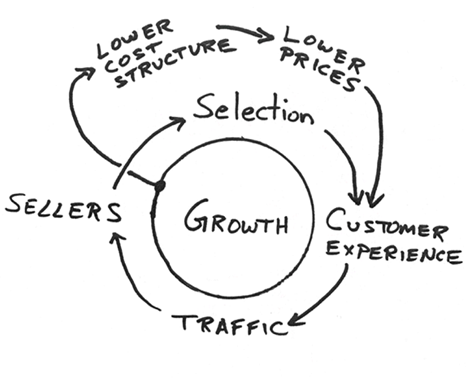
\includegraphics[width=8cm]{media/Fabian-vicious-cycle.png}
        \caption{Amazon's Vicious Cycle}
        \label{vicious-cycle}
        \bildquelle Jeff Bezos, September 2001 %Learn from the Bezos Virtuous Cycle: Leverage and Invest in Infrastructure, www.zentail.com, abgerufen August 2020% https://tinyurl.com/yyu2zz29 DATUM???
    \end{center}
\end{figure} 

Dabei schafft breit gefächerte Produktsegment(Selection) eine positive Kundenerfahrung(Customer Experience), die weitere Verkäufe und Verbreitung durch z. B. Empfehlungen(Traffic) hervorruft. Durch diese hohe Kundenanzahl ist die Plattform wiederrum attraktiver für Drittanbieter und Herstellern(Sellers), die weitere Produkte anbieten und das Produktsegment erweitern. Dieser Teil ist an sich nicht wirklich außergewöhnlich, da viele andere Onlineanbieter eine ähnliche Strategie verfolgen. Jedoch hebt sich Amazon damit ab, ungewöhnlich hohe Summen zu investieren, um Kosten(Lower cost structure) und somit auch Produktpreise(Lower prices) zu senken\cite[S. 26f]{Graf}. Amazon schaffte so auch ein neues Kundenverhalten, das "Amazon Commerce" - Graf und Schneider beschreiben es in ihrem Buch als ein

\begin{quote}
    "[...] komplett neues Kaufverhalten, das sich nicht mehr an Anbietern oder konkreten Produkten orientiert, sondern allein am Zweck [...], den das gewünschte Produkt erfüllen soll."\cite[S. 42]{Graf}
\end{quote}

Die genannten Punkte ermöglichten es Amazon, sich als weltweit bekannten und benutzten Onlineversandhandel zu etablieren - jedoch haben sie auch einige Probleme hervorgerufen. Beispielsweise führte die konstante Niedrigpreispolitik\cite[Abb. 5]{Desjardins} zum Einsparen von Ausgaben in fast allen Gebieten - auch im Bezug auf Angestellte\cite[S. 6]{Apicella}. \iffalse Amazon’s Haupteinnahmequelle ist mit 84\% der Einnahmen zweifelsfrei der Onlinehandel und -versand\cite[Abb. 5]{Desjardins} - und genau dieser hat in den letzten Jahren einige Probleme hervorgerufen. Bespielsweise führt die Verkauffstrategie Amazons, Produkte so billig wie möglich und mit kostenlosem Versand anzubieten, um mehr Käufer anzusprechen\cite{Quartz}, zum Einsparen von Ausgaben in fast allen Gebieten - auch im Bezug auf Arbeiter\cite[S. 6]{Apicella}.\fi So werden insbesondere in der Weihnachtszeit Leiharbeiter eingestellt. In der ARD-Reportage "Ausgeliefert! Leiharbeiter bei Amazon" wird 2013 gezeigt, wie deren Arbeitsalltag aussah: Zu siebt wird in einer Ferienwohnung übernachtet, oft bekommen die Angestellten nur wenige Stunden Schlaf. Jeden Tag aufs neue ist es unsicher, ob man gebraucht wird - wenn nicht, gibt es keinen Lohn. Mitarbeiter der Dienstleistungsgewerkschaft Ver.di und Amazons erklären, dass 2013 in Koblenz circa 3100 von 3300 Arbeitern befristet angestellt waren\cite{Ausgeliefert}.
Außerdem existiert ein hoher Grad an Überwachung und Kontrollen, wie Apicella in ihrer Studie andhand der Stadt Leipzig beschreibt\cite[S. 29]{Apicella}:
\begin{quote}
"Die Verkaufsarbeit durchläuft dabei einen Prozess der [...] vollständige[n] Überwachung und Disziplinierung der Beschäftigten[...]."
\end{quote}
Dementsprechend sind Streiks bei Amazon keine Seltenheit: Beispielsweise streikten Angestellte in Deutschland zwei Monate nach der besagten Reportage unter dem Motto "Wir sind keine Roboter" gegen niedrige Löhne, befristete und schlechte Arbeitsverhältnisse sowie die starke Digitalisierung der Arbeit\cite[S. 6]{Apicella}. Amazon reagierte in den folgenden Jahren mit mehreren Lohnerhöhungen, jedoch exestieren noch vereinzelt Streiks\cite{JGraf}.

Da in Folge der Corona-Krise im 1. Quartal von 2020 die Verkäufe um 32\% stiegen, bekamen Angestellte eine weitere Lohnerhöhung. Zusätzlich wurden 175000 neue Stellen ausgeschrieben - nicht nur, weil mehr Arbeiter als vorher gebraucht werden, sondern auch weil einige Angestellte aufgrund von "unsicheren Bedingungen" zu Hause geblieben sind bzw. dies immer noch tun\cite{Theweek}.

Innerhalb der letzen 26 Jahre hat Amazon sich von einem Online-Buchhandel zu einem weltweiten Onlinehändler fast alle Produktklassen entwickelt. Außerdem bietet die Firma heute auch andere Dienste an, wie z. B. Cloud Computing mit \ac{AWS}. Jedoch steht das Unternehmen bezüglich der Arbeitsbedingungen seit fast einem Jahrzehnt in der Kritik.

%dritanbieter: so kann amazon ein noch breeiteres produktsegment anbieten, während probleme wie kapitalbildung und lagern an händler auszulagern + provision: ecom Buch S 50

            
        \subsection{Einfluss auf das Konsumverhalten } %neu: das Konsumverhalten und der Einfluss des Onlinehandels
            Der Ablauf von Kaufprozessen hat sich in den letzten Jahrzehnten unter Einfluss des Onlinhandels stark geändert. Insbesondere Amazon hat sich als Händler mit niedrigen Preisen und einer sehr großen Auswahl von neuen sowie gebrauchten Produkten weltweit als Verkaufsplattform etabliert. Mithilfe dieser Kombination kann Amazon, im Gegensatz zu anderen Plattformen wie Ebay als Haupteinkaufsmöglichkeit benutzt werden, was wiederrum anderer Online-Konkurrenz und dem stationären Einzelhandel schadet.


%Neben Ebay, welches sich ausschließlich auf Drittanbieter fokussiert, konnte sich nur ein anderes Unternehmen im Onlineverkauf aller Branchen etablieren: Abiexpress, welches noch niedirgere Preise durch Direktverkauf von Herstellern ermöglicht. \emerald 345
Der Hauptgrund für diesen Wandel ist wahrscheinlich, dass bei den meisten Verbrauchsgütern die in [4] beschriebenen Vorteile des stationären Handels\cite[S. 2]{Maier}, hauptsächlich die Beratung und das direkte Betrachten des Produktes, nur wenig Nutzen finden. So ist z. B. beim wiederholten Kaufen von Shampoo, Rasierklingen o. ä. das Produkt schon bekannt und kann problemlos Online bestellt werden. 

\iffalse
    über zeit unkomplizierter geworden
    
    verbilligung des onlinehandels > prime-verlust
    amazon = vorreiter, aliexpress
    
    aliexpress: direkt von hersteller kaufen (https://www.emerald.com/insight/content/doi/10.1108/S1745-886220180000013014/full/pdf?title=italicamazon-and-alibabaitalic-internet-governance-business-models-and-internationalization-strategies 345)
\fi
Dementsprechend führt die seit Jahrzehnten steigende Relevanz des Onlinehandels zu einem Rückgang der Nachfrage im stationären Vertrieb\cite{Shankar}, die durch die derzeitige Corona-Situation noch etwas verstärkt wird - mehr dazu in Kapitel [4 und 5].

\iffalse
 Vorreiter in sachen niedrige Preise > ist sehr wichtig, weil
   viel einfacher vergelichbar, qualität des Produkts nicht einfach einsehbar: sie muss nicht außergewöhnlich, nur akzeptabel sein - jedoch auch nicht schlecht, da 14-tage-rückgabe ohne angabe eines grundes

 
 S 49 https://edoc.sub.uni-hamburg.de/hcu/volltexte/2017/370/pdf/Ebert_Kirsten.pdf
 danach: modell für veränderung
\fi

            
        \subsection{Onlinehändler als Konkurrenten zu lokalen Händlern}
            \iffalse

billig-entwicklung, konkurrenz muss kosten einsparen -> ausbeutung arbeiter, erdrängung kleinerer Onlinhändler und Geschäfte im ländlichen Raum.? kann man die Allgemeinheit auf Schleusingen übertragen
\fi

        \newpage
            
        
    \section{Wirtschaft} %mit blick auf anbieter: sonst überschneidung mit konsumverhalten
        \subsection{Entwicklung der Wirtschaft}
        \subsection{Auswirkungen auf Konzerne und Umwelt}
        \subsection{Auswirkungen auf Paketdienste}
        \subsection{Folgeänderungen von Import/ Export}
        \newpage
        
    \section{Handeln im Internet}
        \subsection{Marketing}
             % https://books.google.de/books?hl=de&lr=&id=KpvzBQAAQBAJ&oi=fnd&pg=PR5&dq=konsumverhalten+entwicklung&ots=7XtmPqXXmZ&sig=xCkMsXi7Up7jXC479QNXaTYPz3o&redir_esc=y#v=onepage&q=konsumverhalten%20entwicklung&f=false

        \subsection{Bezahlvorgänge}
            \input{exports/Fabian/Handeln-Bezahlvorgänge.tex}
        \newpage
    \bibliography{Literaturverzeichnis}
        \newpage
    \listoffigures
        \newpage
    \input{exports/Abkürzungsverzeichnis.tex}
    \listoftables

\end{document}


%ergenisse: nischenwaren mit onlineversand, oder online-verbund mit anderen\ nitt 63
    %viele einzelhandelsflächen ini der stadt durch insolvenzen
    %mglich: hersteller-fabrik einige km von stadtzentrum, laden in der stad, mit onlineshop
    %stärkere, individiuelle bedürfnisse
    %standort immer wichtiger, am besten shoppingcenter \nitt, 7
    %handwerker, baumarkt, apotheken
    %lebensmittel-liefer-roboter zwar in zukunft denkbar, jedoch noch nicht umsetzbar weil probleme wie vandalismus(unbegründete zerstörung von dingen)
    %stationärer handel hat in vielen gebieten geringe zukunftschancen: er wird zwar überleben, trotzdem ist der einstieg neuer händler um so schwerer - jedoch wird er für eine interesannte innenstadt nicht benötigt
    %attraktionen statt verkauf: zB lasertech
    %oder Gastronomie- und Dienstleistungsangebote (zum Beispiel Frisör, Reinigung, Krankengymnastik, Arztpraxen)
    % oder Bildungs- oder Kulturangeboten wie fahrschule
